\documentclass[twoside,10pt]{article}
\usepackage{amsmath,amsfonts,amsthm,fullpage}
\usepackage{mymath}
\usepackage{algorithm}
\usepackage{algorithmic}
\usepackage{graphicx}
\usepackage{mathtools}

\begin{document}

\title{CS 7641 CSE/ISYE 6740 Homework 1 Report}
\author{Rakesh Surapaneni}
\maketitle

%----------------------------------------------------------------------------------
\section{Programming: Image compression [30 pts]}


\begin{enumerate}
  \item Within the $K$-medoids framework, you have several choices for detailed implementation. Explain how you designed and implemented details of your $K$-medoids algorithm, including (but not limited to) how you chose representatives of each cluster, what distance measures you tried and chose one, or when you stopped iteration.\\
\\
\textbf{ANS:}\\
  Attempts I have failed: 
  \begin{enumerate}
	\item I have tried calculating distance between every pair of point. The time complexity for this operation is O($n^2$) and hence very slow. 
    \item I have also tried cosine distance instead of Euclidean square distance. I have experimented on this since I want to eliminate brightness out of similarity measure(the top part of pics are generally bright). However There are many white spots in the picture after this implementation due to some reason and picture quality is lost. Hence I have to abandon this approach.
  \end{enumerate}
  Final implementation:
  \begin{enumerate}
	\item The distance metrics D is same Euclidean square distance measure which is used in general K-means algorithm. 
    \item To calculate k-medoid instead of k-means, I actually calculate mean of the cluster and find nearest point to the mean. Clearly though this is not most accurate k-medoid, this is better solution due to time complexity issues.
    \item The code runs till the percentage change in overall cost is less than 0.1%
    \item In addition to the percentage change, I have limited number of iterations to 100 to limit the time complexity.
  \end{enumerate}


 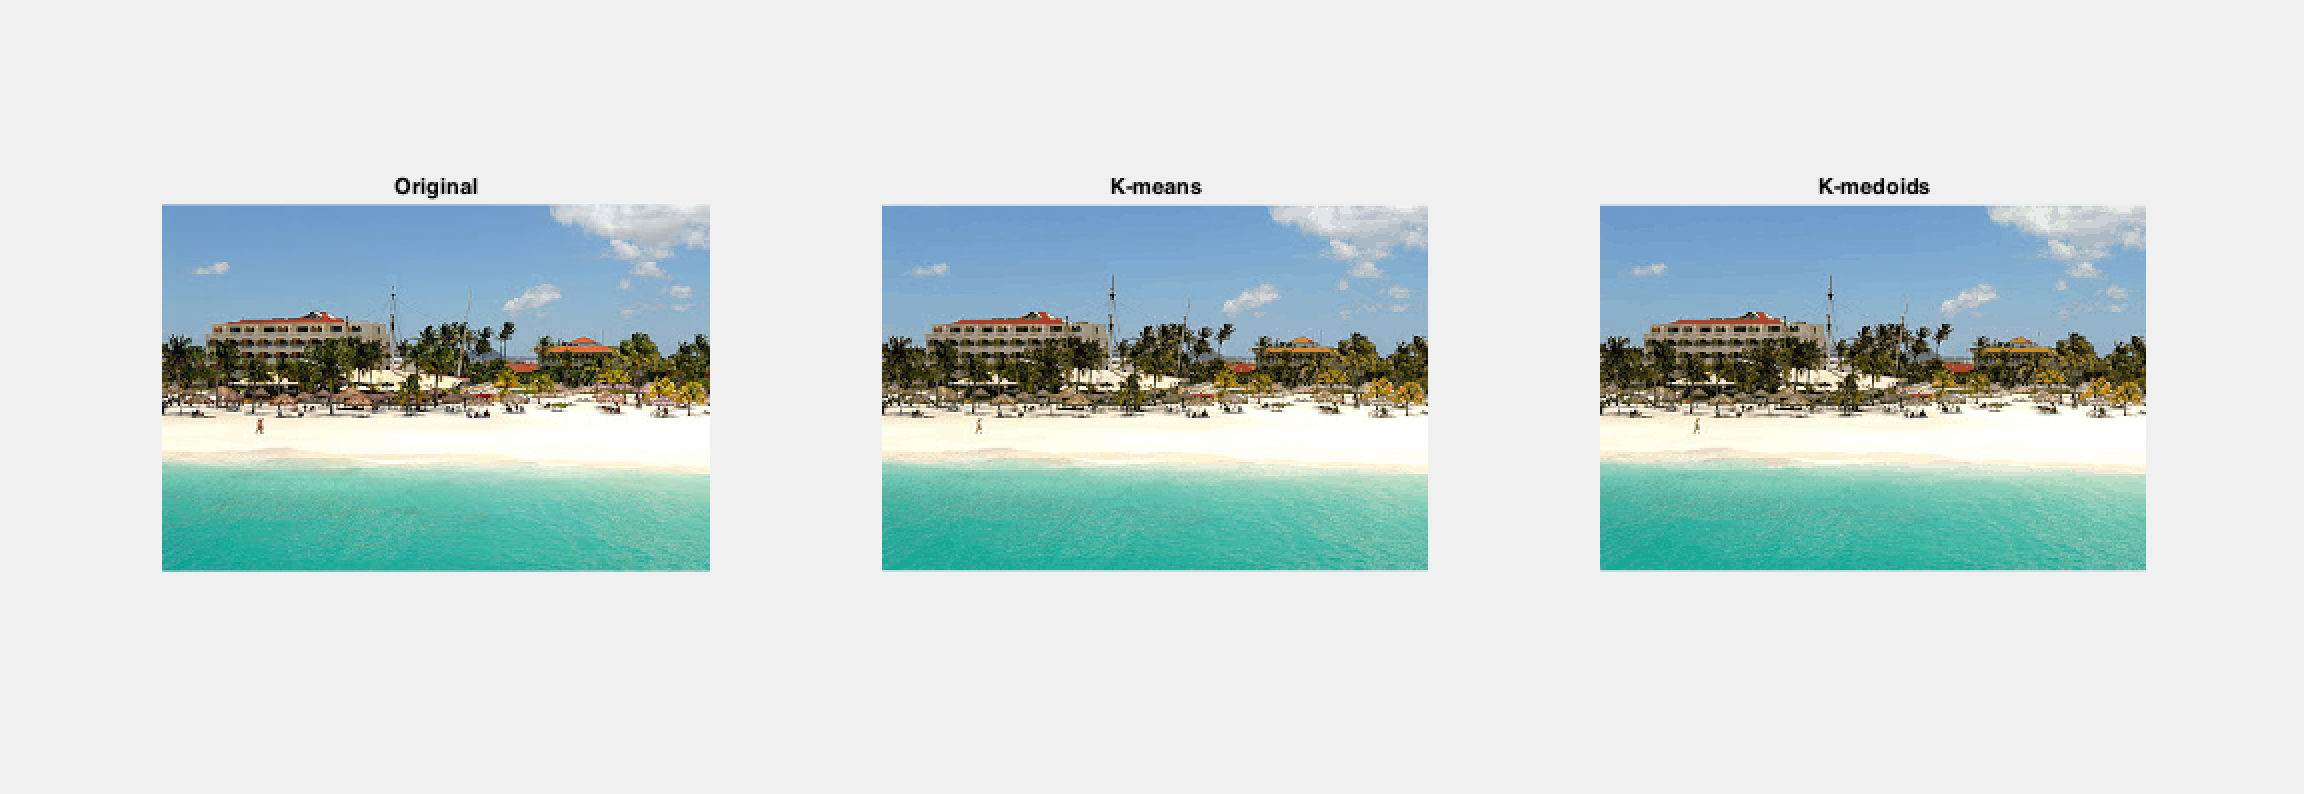
\includegraphics[width=\textwidth,height=\textheight,keepaspectratio]{final_implementation.png}
 Figure 1: The output for K = 100 and final implementation
 
 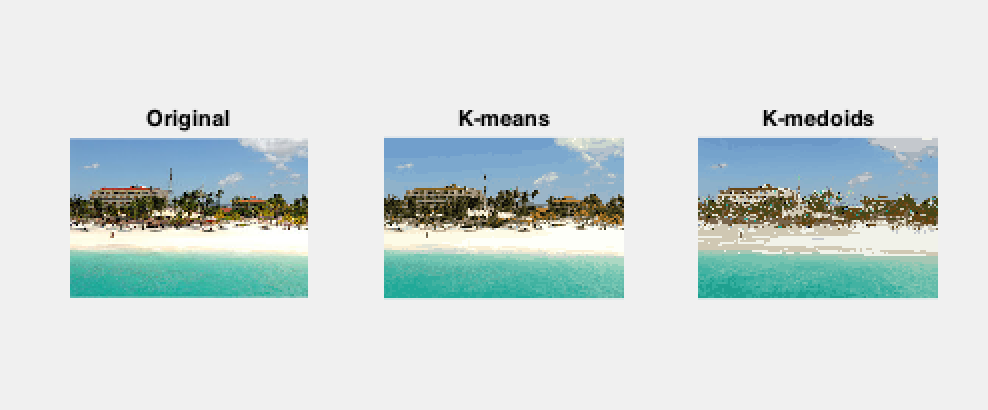
\includegraphics[width=\textwidth,height=\textheight,keepaspectratio]{cosine_distance_implementation.png}
 Figure 1: The output for implementation using cosine distance measure. \\
 The quality decreased due to the white spots in cosine distance metrics based measurement. 
 
\vspace{1cm}
  
  \item Attach a picture of your own. We recommend size of $320 \times 240$ or smaller.\\
  \\
  \textbf{ANS:}\\
  I have used an image "eagle.png" as shown below.\\
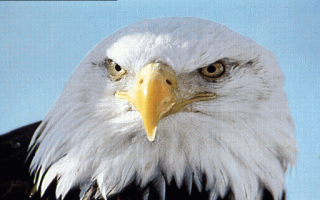
\includegraphics[width=\textwidth,height=\textheight,keepaspectratio]{eagle.png}
  eagle.png\\
  \item Run your $K$-medoids implementation with the picture you chose above, with several different $K$. (e.g, small values like 2 or 3, large values like 16 or 32) What did you observe with different $K$? How long does it take to converge for each $K$?\\
\\
\textbf{ANS:}\\
Table showing time consumed in seconds for various k values for k-means and k-medoids as well.
  \begin{table}[!h]
\centering \small
\begin{tabular}{l|c|c}
  \hline
  K-Value & K-means & K-medoid\\
  \hline \hline
  K = 2 & 11.4 sec & 12.2 sec\\
  K = 3 & 12.6 sec & 13.4 sec\\
  k = 4 & 13.2 & 13.7\\
  k = 10 & 17.1 & 12.8\\
  k = 20 & 61.5 & 14.0\\
  k = 32 & 65.1 & 15.2\\
  k = 64 & 71 & 16.7\\
  k = 100 & 75.2 & 20.8\\
  k = 128 & 75.3 & 100.2\\
  k = 129 & 74 & 18.2\\
  \hline
\end{tabular}
\end{table}\\
\vspace{1cm}
 Surprisingly for lower k, I see k-medoid perform better.\\
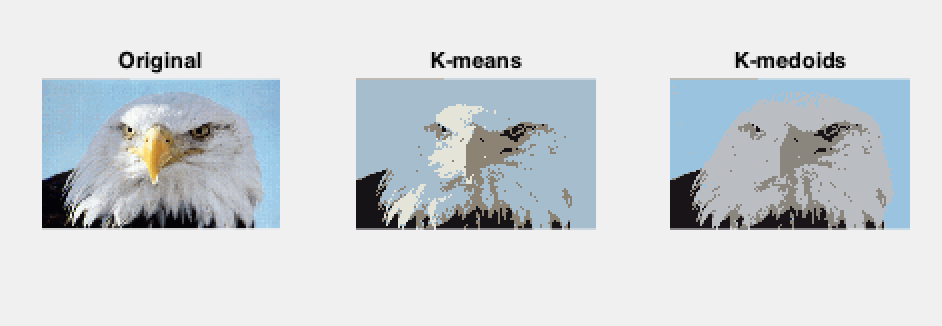
\includegraphics[width=\textwidth,height=\textheight,keepaspectratio]{k_equals_4.png}
  \item Run your $K$-medoids implementation with different initial centroids/representatives. Does it affect final result? Do you see same or different result for each trial with different initial assignments? (We usually randomize initial location of centroids in general. To answer this question, an intentional poor assignment may be useful.)
  \\
\\
\textbf{ANS:}\\
\hspace*{1cm}	It does matter what values the cluster centers are initialized to. I have checked various iterations and based on initial values for each values of k, the variance in picture quality and time taken varies. \\
\hspace*{1cm}   For \textbf{higher values of k}, time taken for the algorithm to run is affected by the initial assignment. For k-medoid algorithm, it takes roughly from 11-18 seconds for k = 20 for different iterations to converge depending on the initial assignment.\\
\hspace*{1cm}   For \textbf{lower values of k}, instead of run time, the performance of algorithm in terms of picture quality is affected. In multiple iterations, I was able to see clear line between eagle and blue space for k= 4 but in some I couldn't.\\
  \item Repeat question 2 and 3 with $K$-means. Do you see significant difference between $K$-medoids and $K$-means, in terms of output quality, robustness, or running time?\\
\\
\textbf{ANS:}\\
\hspace*{1cm} Please look at the solution table in part c to get time stats for k-means algorithm.\\
\hspace*{1cm} For \textbf{lower values for of k}, I see k-means and k-medoids performing almost similarly. However in some cases I was able to clearly see edge in k-medoid algorithms.\\
\hspace*{1cm} For \textbf{higher values of k}, I see k-medoids generally converge faster leading to lower run time compared to k-means.\\
\hspace*{1cm} Again these results are varying for each try and hence too random to compare.\\
\hspace*{1cm} For some strange reason, I see that for \textbf{k= 128}, K-medoids is always taking time around ~100 seconds. I am not sure why this phenomenon is happening though. For \textbf{k = 129}, however it takes only 17 seconds for k-medoid to converge.
\end{enumerate}
\end{document}